\documentclass[conference]{IEEEtran}
\IEEEoverridecommandlockouts

% Packages
\usepackage{cite}
\usepackage{amsmath,amssymb,amsfonts}
\usepackage[dvipsnames]{xcolor}
\usepackage{graphicx}
\usepackage{textcomp}
\usepackage{listings}
\usepackage{subcaption}
\usepackage{multirow}
\usepackage{algorithm}
\usepackage{algpseudocode}
\usepackage{algorithmicx}
\usepackage{url}
\usepackage{caption}
\usepackage{tcolorbox}
\usepackage{hyperref}
\usepackage[T1]{fontenc}
\usepackage{enumitem}

\setlength {\marginparwidth }{2cm}
\usepackage{todonotes}

\hypersetup{hidelinks}
\newcommand{\algorithmautorefname}{Algorithm}
\captionsetup[algorithm]{name=Alg.} 

\tcbuselibrary{listingsutf8}
\newtcbox{\redbox}[1][]{
 on line, 
 boxsep=1pt, 
 left=1pt, 
 right=1pt, 
 top=1pt, 
 bottom=1pt, 
 colframe=red!75!black, 
 colback=red!10, 
 boxrule=0.5pt, 
 rounded corners,
 #1
}

\algrenewcommand\algorithmicindent{0.8em} 



\begin{document}

\title{Algorithm Selection and Auto-Tuning in AutoPas}

\author{
    \IEEEauthorblockN{ Manuel Lerchner}
    \IEEEauthorblockA{
        \textit{Technical University of Munich}\\
        Munich, Germany}
}

\maketitle

\begin{abstract}
    Molecular dynamics (MD) simulations face significant computational challenges that require highly optimized simulation engines to deal with the enormous number of particles present in modern simulations. Naturally, researchers have put much effort into developing algorithms and frameworks that can efficiently simulate these systems. This paper focuses on the AutoPas framework, a modern MD framework that uses dynamic optimization techniques to achieve high performance in complex simulation scenarios. We compare AutoPas with other prominent MD engines, such as GROMACS, LAMMPS, and ls1 mardyn, and investigate a possible improvement to AutoPas' auto-tuning capabilities by introducing an early stopping mechanism to reduce the overhead of parameter space exploration. Our evaluation shows that an early stopping mechanism can reduce the total simulation time by up to 18.9\% when using the predictive tuning strategy.
\end{abstract}

\begin{IEEEkeywords}
    molecular dynamics, auto-tuning, autopas, early-stopping, gromacs, lammps, ls1 mardyn
\end{IEEEkeywords}

\section{Introduction}

Molecular dynamics simulations represent a computational cornerstone in various scientific fields, from materials science to biochemistry. These simulations typically use complex and computationally intensive interaction models acting on enormous numbers of particles to ensure accurate results. Therefore, the computational complexity of these simulations grows rapidly with the number of particles, requiring highly optimized simulation engines to guarantee feasible simulation times. Prominent optimization techniques used in modern molecular dynamics (MD) engines fall into two main categories: static and dynamic optimization.

Static optimizations rely on predefined configurations and performance models, often fine-tuned for specific hardware architectures. They are selected before the simulation begins and remain constant throughout the simulation. Static optimizations include automatic optimizations performed by modern compilers (e.g., loop unrolling, inlining, auto-vectorization), conditional compilation based on the target hardware (e.g. SIMD)~\cite{Gratl2019AutoPas}, or manual selection of simulation parameters based on expert knowledge.

Dynamic optimizations adjust parameters based on the current simulation state and the actual hardware performance. Unlike static optimizations, dynamic optimizations allow for adjustments throughout the simulation. This approach is favourable, as the engine can adapt and optimize itself without external intervention and can adapt itself to the progressing simulation. However, dynamic optimizations come at the cost of increased complexity and potential overhead, as the engine must periodically re-evaluate its configuration based on the current simulation state.

In particular, we will focus on the auto-tuning capabilities of AutoPas, a modern MD framework that focuses on dynamic optimization techniques to achieve high performance in complex and possibly changing simulation scenarios. We compare AutoPas with other prominent MD engines, such as GROMACS, LAMMPS, and ls1 mardyn, and investigate a possible improvement to AutoPas' auto-tuning capabilities by introducing an early stopping mechanism to reduce the overhead of parameter space exploration.


\section{AutoPas}

AutoPas was developed on the basis of creating an efficient particle / N-Body simulation engine applicable to a wide range of applications~\cite{Tchipev2020}. Therefore, AutoPas is built on a modular software architecture that allows different algorithms and data structures to be used interchangeably in the underlying simulation engine. AutoPas acts as a middleware between the simulation code provided by the user and various implementations of algorithms and data structures capable of solving N-Body problems efficiently. As all implementations are (mostly) interchangeable, AutoPas can provide a wide range of so called \textit{Configurations} which fully describe the internal implementation of the engine.
To lift the burden of selecting suitable configurations from the user, and to allow for dynamic optimization, AutoPas provides an auto-tuning framework that periodically evaluates different configurations and selects the best one based on certain performance metrics. This selection is performed by so-called \textit{TuningStrategies} that try to prune the search space of possible configurations according to a specific strategy. \autoref{fig_architecture} shows a high-level overview of the AutoPas library structure.

\begin{figure}[H]
    \centering
    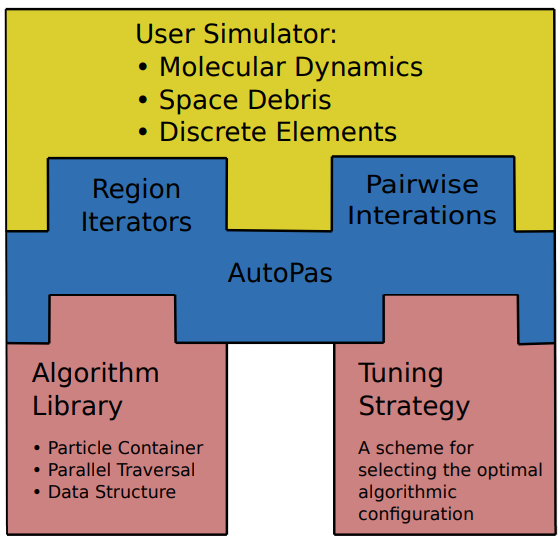
\includegraphics[width=2.2in]{figures/AutoPasLibraryStructure.png}
    \caption{AutoPas Library Structure as depicted by~\cite{Newcome2023Poster}}
    \label{fig_architecture}
\end{figure}

\subsection{Algorithm Library}

All different algorithmic implementations for solving N-Body problems are part of the so-called \textit{Algorithm Library} of AutoPas. The \textit{Algorithm Library} contains different implementations for certain key aspects of the simulation, such as neighbor identification, traversal patterns, memory layouts and optimization techniques.

A combination of different implementations for each key aspect of the simulation is called a \textit{Configuration}. Currently AutoPas supports the six tunable parameters: \textit{Container}, \textit{Traversal}, \textit{Load Estimator}, \textit{Data Layout}, \textit{Newton 3}, and \textit{Cell Size Factor}.

As implementations for a tunable parameter are (mostly) interchangeable, it is straightforward to create new, potentially hardware-specific, implementations for each key aspect of the simulation, allowing for both a bigger search space of possible configurations and performance portability across different hardware platforms~\cite{Tchipev2020}. Another benefit of this modular approach is presented with the implicit backward compatibility of the interchangable implementations. With the ever growing number of configurations, it is possible to test the feasibility of older implementations under new hardware~\cite{Tchipev2020}.

The next sections will provide a detailed overview of prominent tunable parameters and the different implementations available in the AutoPas framework.

\begin{description}[style=nextline]
    \item[Container]

        Containers are responsible for storing the particles of the simulation such that relevant neighbor particles can be determined efficiently. As AutoPas focuses on short-range interactions with a force cutoff radius $r_c$, neighbor identification using just $O(N)$ distance calculations is possible~\cite{Gratl2019AutoPas}, drastically reducing the computational complexity of the simulation. \autoref{fig_containers} shows important container types used in AutoPas.

        \begin{figure}[h]
            \centering
            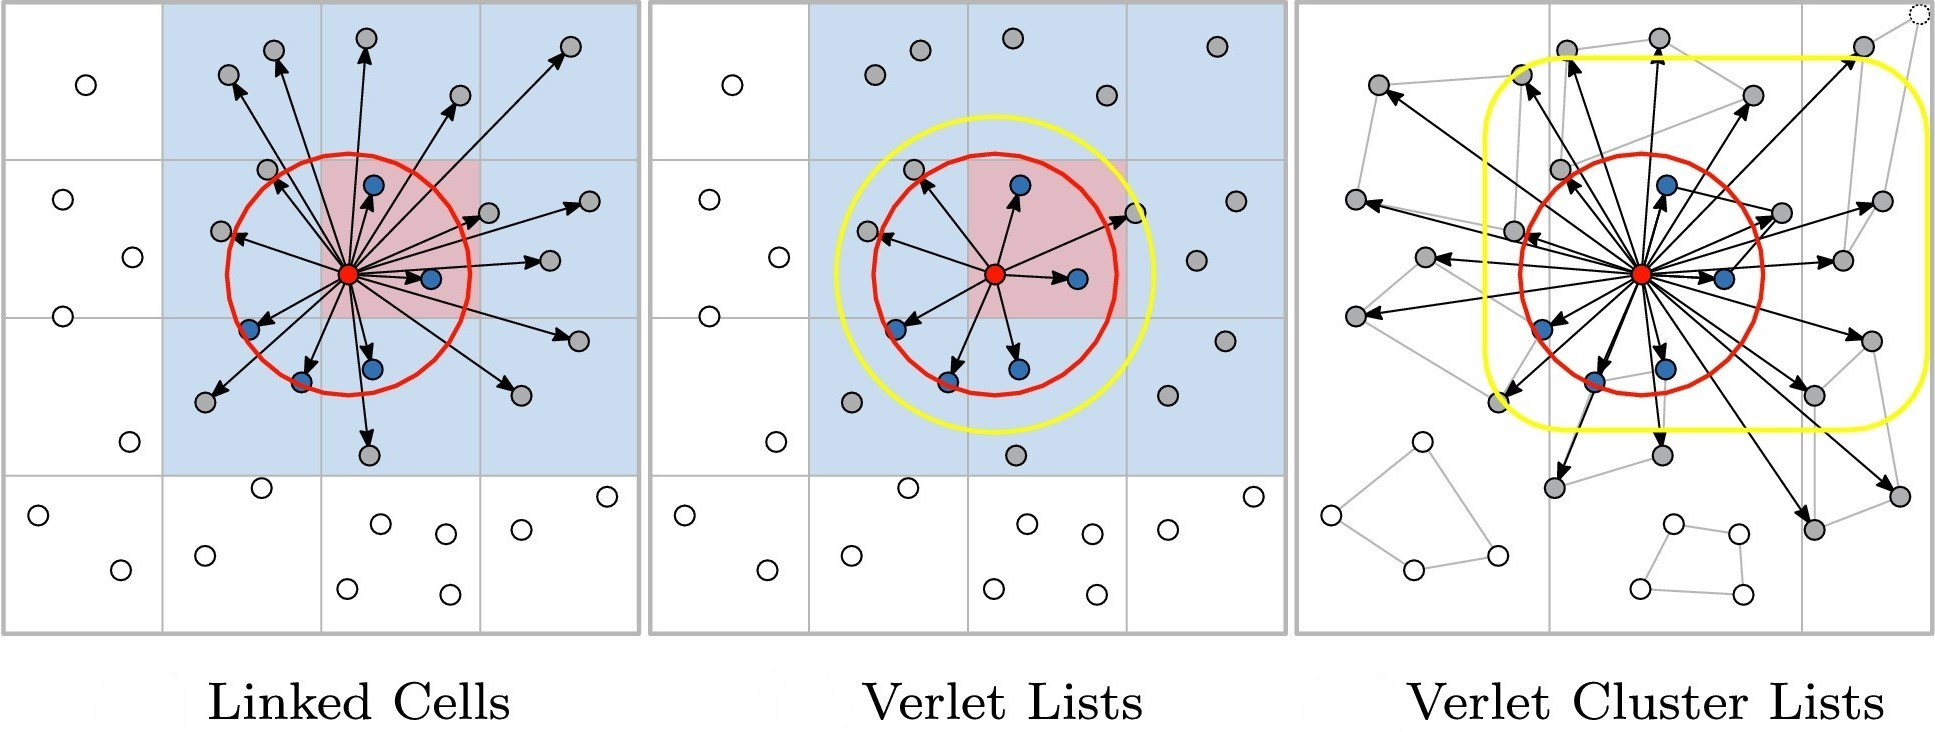
\includegraphics[width=\columnwidth]{figures/containers.jpg}
            \caption{Important Container Types as depited by~\cite{Gratl2022AutoPas}. The cutoff radius $r_c$ is shown using a red circle. The arrows represent distance checks between particles. Only particles shown in blue contribute to the final force calculation.}
            \label{fig_containers}
        \end{figure}

        \begin{description}[style=nextline, font=\itshape\mdseries]
            \item[LinkedCells]
                The LinkedCells algorithm maintains a grid of cells with a length of $r_c$ (when $cellSizeFactor = 1$). When calculating forces for a particle, only particles in neighboring cells (depicted in blue) need to be considered, as all other particles are guaranteed to be outside the cutoff radius.

                LinkedCell casues many spurious distance calculations (shown by many arrows to gray particles in the figure). As particles for a cell can be stored together in memory, LinkedCells are however very cache-friendly~\cite{Gratl2022AutoPas}.

            \item[VerletLists]
                The VerletList algorithm uses a second radius $r_v = {r_c} + \Delta_s$ (yellow circle) and considers all particles within this radius as potential neighbors. Contrary to LinkedCells, each particle maintains its own list of potential neighbors. As the bigger radius $r_v$ provides a buffer region, it is possible to only rebuild the neighbor-list every $n$ simulation steps, as long as no particle can move from outside $r_c + \Delta_s$ to inside $r_c$ unnoticed~\cite{NEWCOME2023115278}.

                VerletLists have very few spurious distance calculations but result in far higher memory consumptions and are less cache-friendly~\cite{Gratl2022AutoPas}, resulting in inefficient vectorization~\cite{PALL20132641}.

            \item[VerletClusterList]
                The Verlet Cluster Lists algorithm improves on the VerletList algorithm by grouping particles into clusters of size $M$ ($M=4$ in the figures). Maintaining the neighbor list and keeping track of buffer regions is done on a cluster level, reducing the memory overhead of the VerletList algorithm.

                As all particles in overlapping clusters need to be considered for the force calculation, the number of spurious distance calculations increases again. When $M$ is chosen in accordance with the SIMD width of the system, efficient vectorization is possible~\cite{Gratl2022AutoPas}.
        \end{description}


    \item[Newton 3]
        Applying Newton's third law to the force calculations allows for a reduction of the number of force calculations by half, as the calculated force between two particles can be reused for the second particle. The optimization can be enabled or disabled in accordance with the interaction model and the traversal pattern.

    \item[Traversal]
        Traversals are responsible for iterating over the particles in the simulation and calculating their interactions in a shared-memory environment~\cite{SECKLER2021101296}. The traversal pattern determines to which extent force calculations can be parallelized and whether optimizations, such as Newton 3, can be applied. \autoref{fig_traversals} shows important traversal patterns used in AutoPas.

        \begin{figure}[H]
            \centering
            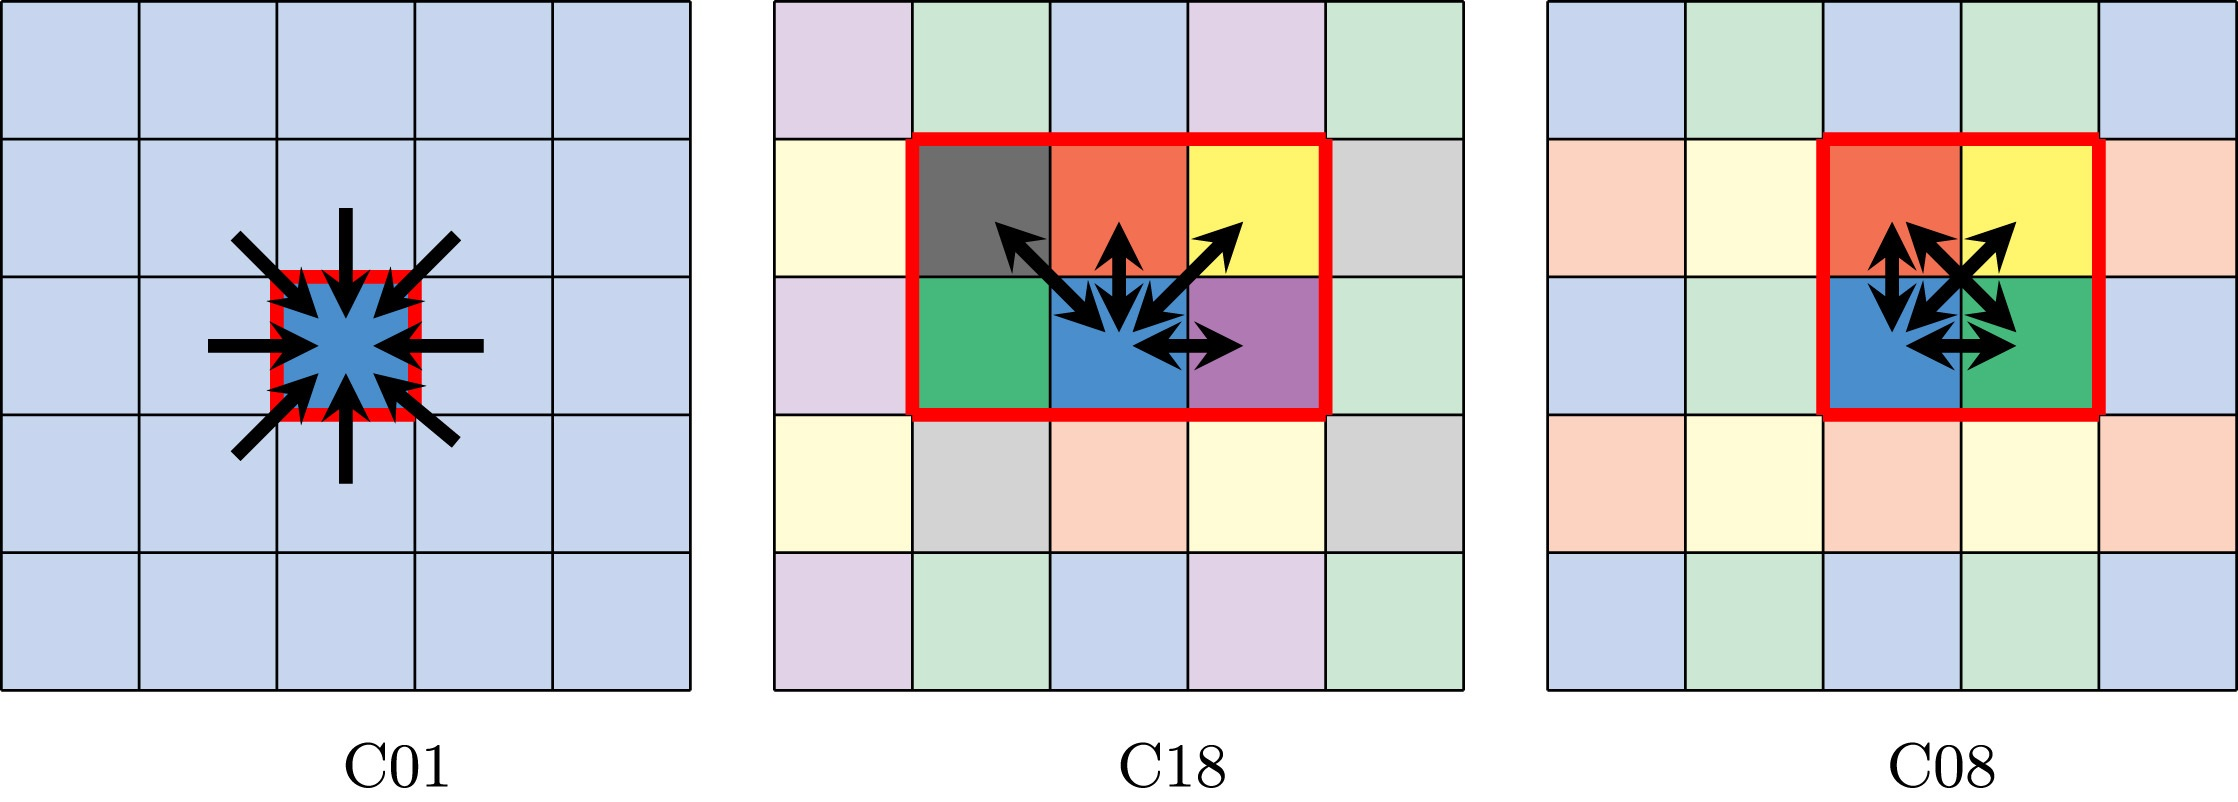
\includegraphics[width=\columnwidth]{figures/traversals.jpg}
            \caption{Important Traversal Types as depicted by~\cite{NEWCOME2023115278}.}
            \label{fig_traversals}
        \end{figure}

        \begin{description}[style=nextline, font=\itshape\mdseries]
            \item[C01]
                The C01 traversal pattern processes each cell independently, resulting in an embarrassingly parallel traversal pattern. Newton 3 can not be used in this traversal pattern, as neighboring cells can be processed in parallel, which could result in race conditions. No synchronization between cells is required, resulting in a high degree of parallelism.
            \item[C18]
                The C18 traversal pattern uses color assignments to ensure that no race conditions occur when using Newton 3. \autoref{fig_traversals} shows that the cells are colored in a regular pattern, such that no two cells of the same color share common neighbors. To ensure that forces are only applied once when using Newton 3, each cell only applies forces to cells \textit{above} and \textit{right} of it.

                During the force calculation, all available threads are working on a single color, and can therefore safely apply the force obtained by Newton 3 on neighboring cells. \\
                The color groups must be processed sequentially, resulting in 18 synchronization points. Each color can however be fully processed in parallel, still resulting in a high overall degree of parallelism ~\cite{NEWCOME2023115278}.
            \item[C08]
                traversal pattern is similar to the C18 traversal pattern but uses a different coloring scheme with only eight colors. This reduces the number of synchronization points, resulting in a higher degree of parallelism at the cost of more scheduling overheads~\cite{NEWCOME2023115278}.
        \end{description}

    \item[Data Layout]
        The Data Layout describes how the particle data is stored in memory. Possible choices are \textit{SoA} (Structure of Arrays) and \textit{AoS} (Array of Structures). \textit{SoA} is typically more cache-friendly and allows for better vectorization. However, it causes information about a single particle to be spread across multiple memory locations. \textit{AoS} on the other hand stores all information about a single particle together but prohibits efficient vectorization as filling vector registers requires gathering data from multiple memory locations.
\end{description}


\subsection{Auto-Tuning Framework}

As described previously, manual selection of suitable implementations for each tunable parameter is a daunting task and would require extensive domain knowledge that is challenging to acquire and maintain under the constantly changing software and hardware landscape. To address this issue, AutoPas performs automated algorithm selection to maximize specific performance metrics, such as simulation speed or energy efficiency~\cite{Gratl2022AutoPas}. Internally AutoPas periodically initiates so-called \textit{tuning-phases} in which promising configurations are evaluated, in order to determine the best Configuration for the current simulation state~\cite{Gratl2019AutoPas}. The winning Configuration is then used until the next tuning phase is initiated.

The key to efficient tuning phases is the ability to efficiently determine promising configurations. The naive approach of evaluating all possible configurations is infeasible in practice, as many of the naively evaluated configurations turn out to be orders of magnitude slower than the best-known Configuration, thus causing a drastic increase of the total simulation time~\cite{endreport.pdf}\cite{Manuel_Lerchner_Thesis.pdf}.
As AutoPas is developed further and new implementations are added to the algorithm library, the number of possible configurations will steadily increase, constantly exacerbating the problem of evaluating all configurations naively.

AutoPas attempts to mitigate this problem by using Tuning Strategies to select promising configurations. Tuning strategies are tasked with pruning enough configurations to make the tuning phase feasible, but not too many, to avoid missing the optimal Configuration.
Tuning strategies balance the trade-off between potentially finding a better configuration and the cost of potentially encountering worse configurations during further exploration~\cite{Newcome2023Poster}.


\todo{Add some tuning strategies}

\section{Benefits of AutoTuning}

\section{Drawbacks of AutoTuning}

Even though AutoPas is capable of performing periodic auto-tuning, it is often beneficial to just execute a single tuning phase right at the beginning of the simulation as performing additional tuning phases could cause unnecessary overhead.

Many scenarios, especially homogeneous ones with simple interaction models, tend to behave fairly stable over time which makes it very likely that the best Configuration found in the first tuning phase remains the best Configuration for the entire simulation.

Further evaluation of training data of \texttt{md-flexible} simulations obtained in \cite{lerchner2024} shows that only three out of 184 runs show any changes in the best Configuration after the first tuning phase. This indicates that all currently provided example scenarios of \texttt{md-flexible} are incapable of demonstrating the benefits of periodic re-tuning.

More complex scenarios, most likely involving multiple nodes and inhomogeneous particle distributions, are necessary to fully demonstrate the benefits of periodic re-tuning. Simulating inhomogeneous scenarios using multiple nodes can cause the load to be distributed unevenly across the nodes and time steps, further increasing the potential benefits of periodically re-tuning the Configuration on each node.


\newpage
\newpage


\section{Early Stopping Optimization}

As identified by~\cite{autopas_issue673}\cite{endreport.pdf}\cite{Manuel_Lerchner_Thesis.pdf}, overhead caused by evaluating suboptimal configurations during the tuning phase can be a significant bottleneck in the performance of the AutoPas framework. Even though the tuning strategies employed by AutoPas are highly efficient, they still sometimes suggest suboptimal configurations. Rule-driven tuning strategies such as \textit{RuleBasedTuning} and \textit{FuzzyTuning} can mitigate this problem to some extent, but due to the complexity of particle simulations, those rule bases are expected to be highly incomplete.

All mentioned sources suggest that some form of \textit{early stopping} mechanism could benefit the AutoPas framework. The primary goal of such a mechanism would be to detect tuning iterations that take much longer than the currently best-known Configuration and stop the evaluation of those configurations early. There are two approaches to this problem:

\begin{itemize}
    \item \textbf{Stopping Further Samples}\\
          AutoPas supports testing a certain configuration multiple times to account for the inherent noise in performance measurements. A simple way to implement early stopping would be to stop the evaluation of further samples of a configuration as soon as it is clear that the performance is significantly worse than the best-known Configuration.

          The implementation of this approach is relatively simple, but may not be as effective as the second approach, as it still requires fully evaluating the first sample of a bad configuration.
    \item \textbf{Interrupting the Evaluation}\\
          A more fine-grained approach, proposed in~\cite{endreport.pdf} could interrupt the evaluation of a long running configuration during its execution.

          The Implementation of this approach requires a big rewrite of the current AutoPas framework, and would require the user to implement synchronizations between multiple nodes in an MPI environment.
\end{itemize}

To get a first impression of the potential benefits of an early stopping mechanism, we implemented the first approach into the AutoPas framework. The changes to the existing codebase are minimal, as the early-stopping mechanism can be implemented using existing functionality. \autoref{alg_early_stopping} shows the main changes to the \texttt{AutoTuner.cpp} file.

Both described approaches require a user-defined threshold for the maximum allowed slowdown of a configuration before it should be stopped. As finding optimal thresholds is a non-trivial task and may depend on the simulation scenario and the tuning strategy, suitable thresholds will be determined empirically in \autoref{sec:evaluation}.

\subsection{Implementation}
The early stopping mechanism is triggered by the new \texttt{evaluateConfiguration} function, which is called after the performance of a configuration has been measured. The function compares the performance of the current Configuration to the best-known performance encountered so far. If the performance of the current Configuration is significantly worse than the best-known performance, the \texttt{abort} flag is set to true, causing the \texttt{GetNextConfiguration} function to select a new configuration on the next call.

\begin{algorithm}[H]
    \small
    \caption{Early Stopping Algorithm in AutoPas}
    \label{alg_early_stopping}
    \begin{algorithmic}[1]
        \Procedure{evaluateConfiguration}{performance}
        \State $fastestTime \gets \min(fastestTime, performance)$
        \State $slowdownFactor \gets \frac{performance}{fastestTime}$
        \If{$slowdownFactor > maxAllowedSlowdown$}
        \State $abort \gets true$
        \EndIf
        \EndProcedure

        \vspace{0.5em}

        \Procedure{GetNextConfiguration}{}
        \If{not $inTuningPhase$}
        \State \Return ($currentConfig, false)$
            \ElsIf{$numSamples$ $<$ $maxSamples$ \redbox{\textbf{and} not $abort$}}
            \State \Return $(currentConfig, true)$
            \Else
            \State $stillTuning \gets \Call{tuneConfiguration}{~}$
            \State \Return $(newConfig, stillTuning)$
        \EndIf
        \EndProcedure
    \end{algorithmic}

\end{algorithm}



\subsection{Evaluation: Exploding Liquid Simulation}
\label{sec:evaluation}

To evaluate the performance of the early stopping mechanism and to determine suitable thresholds for the maximum allowed slowdown, we perform a benchmark using the \textit{Exploding Liquid} scenario provided by the \texttt{md-flexible} framework. The simulation consists of 1764 initially close-packed particles that are simulated with a Lennard-Jones potential. During the simulation, the particles rapidly expand outwards and eventually hit the simulation boundaries\footnote{A simulation video can be found at \url{https://youtu.be/u7TE5KiSQ08}}.

All benchmarks are performed on a single node of the CoolMUC2\footnote{CoolMUC-2 is a supercomputer at the Leibniz Supercomputing Centre in Garching, Germany. See: https://doku.lrz.de/coolmuc-2-11484376.html} supercomputer using 14 threads. To ensure reproducibility, all runs are repeated three times.

\subsubsection{Full Search}

The resulting performance when using the FullSearch strategy in combination with the early stopping mechanism is shown in \autoref{fig:full_search}.

\begin{figure}[H]
    \centering

    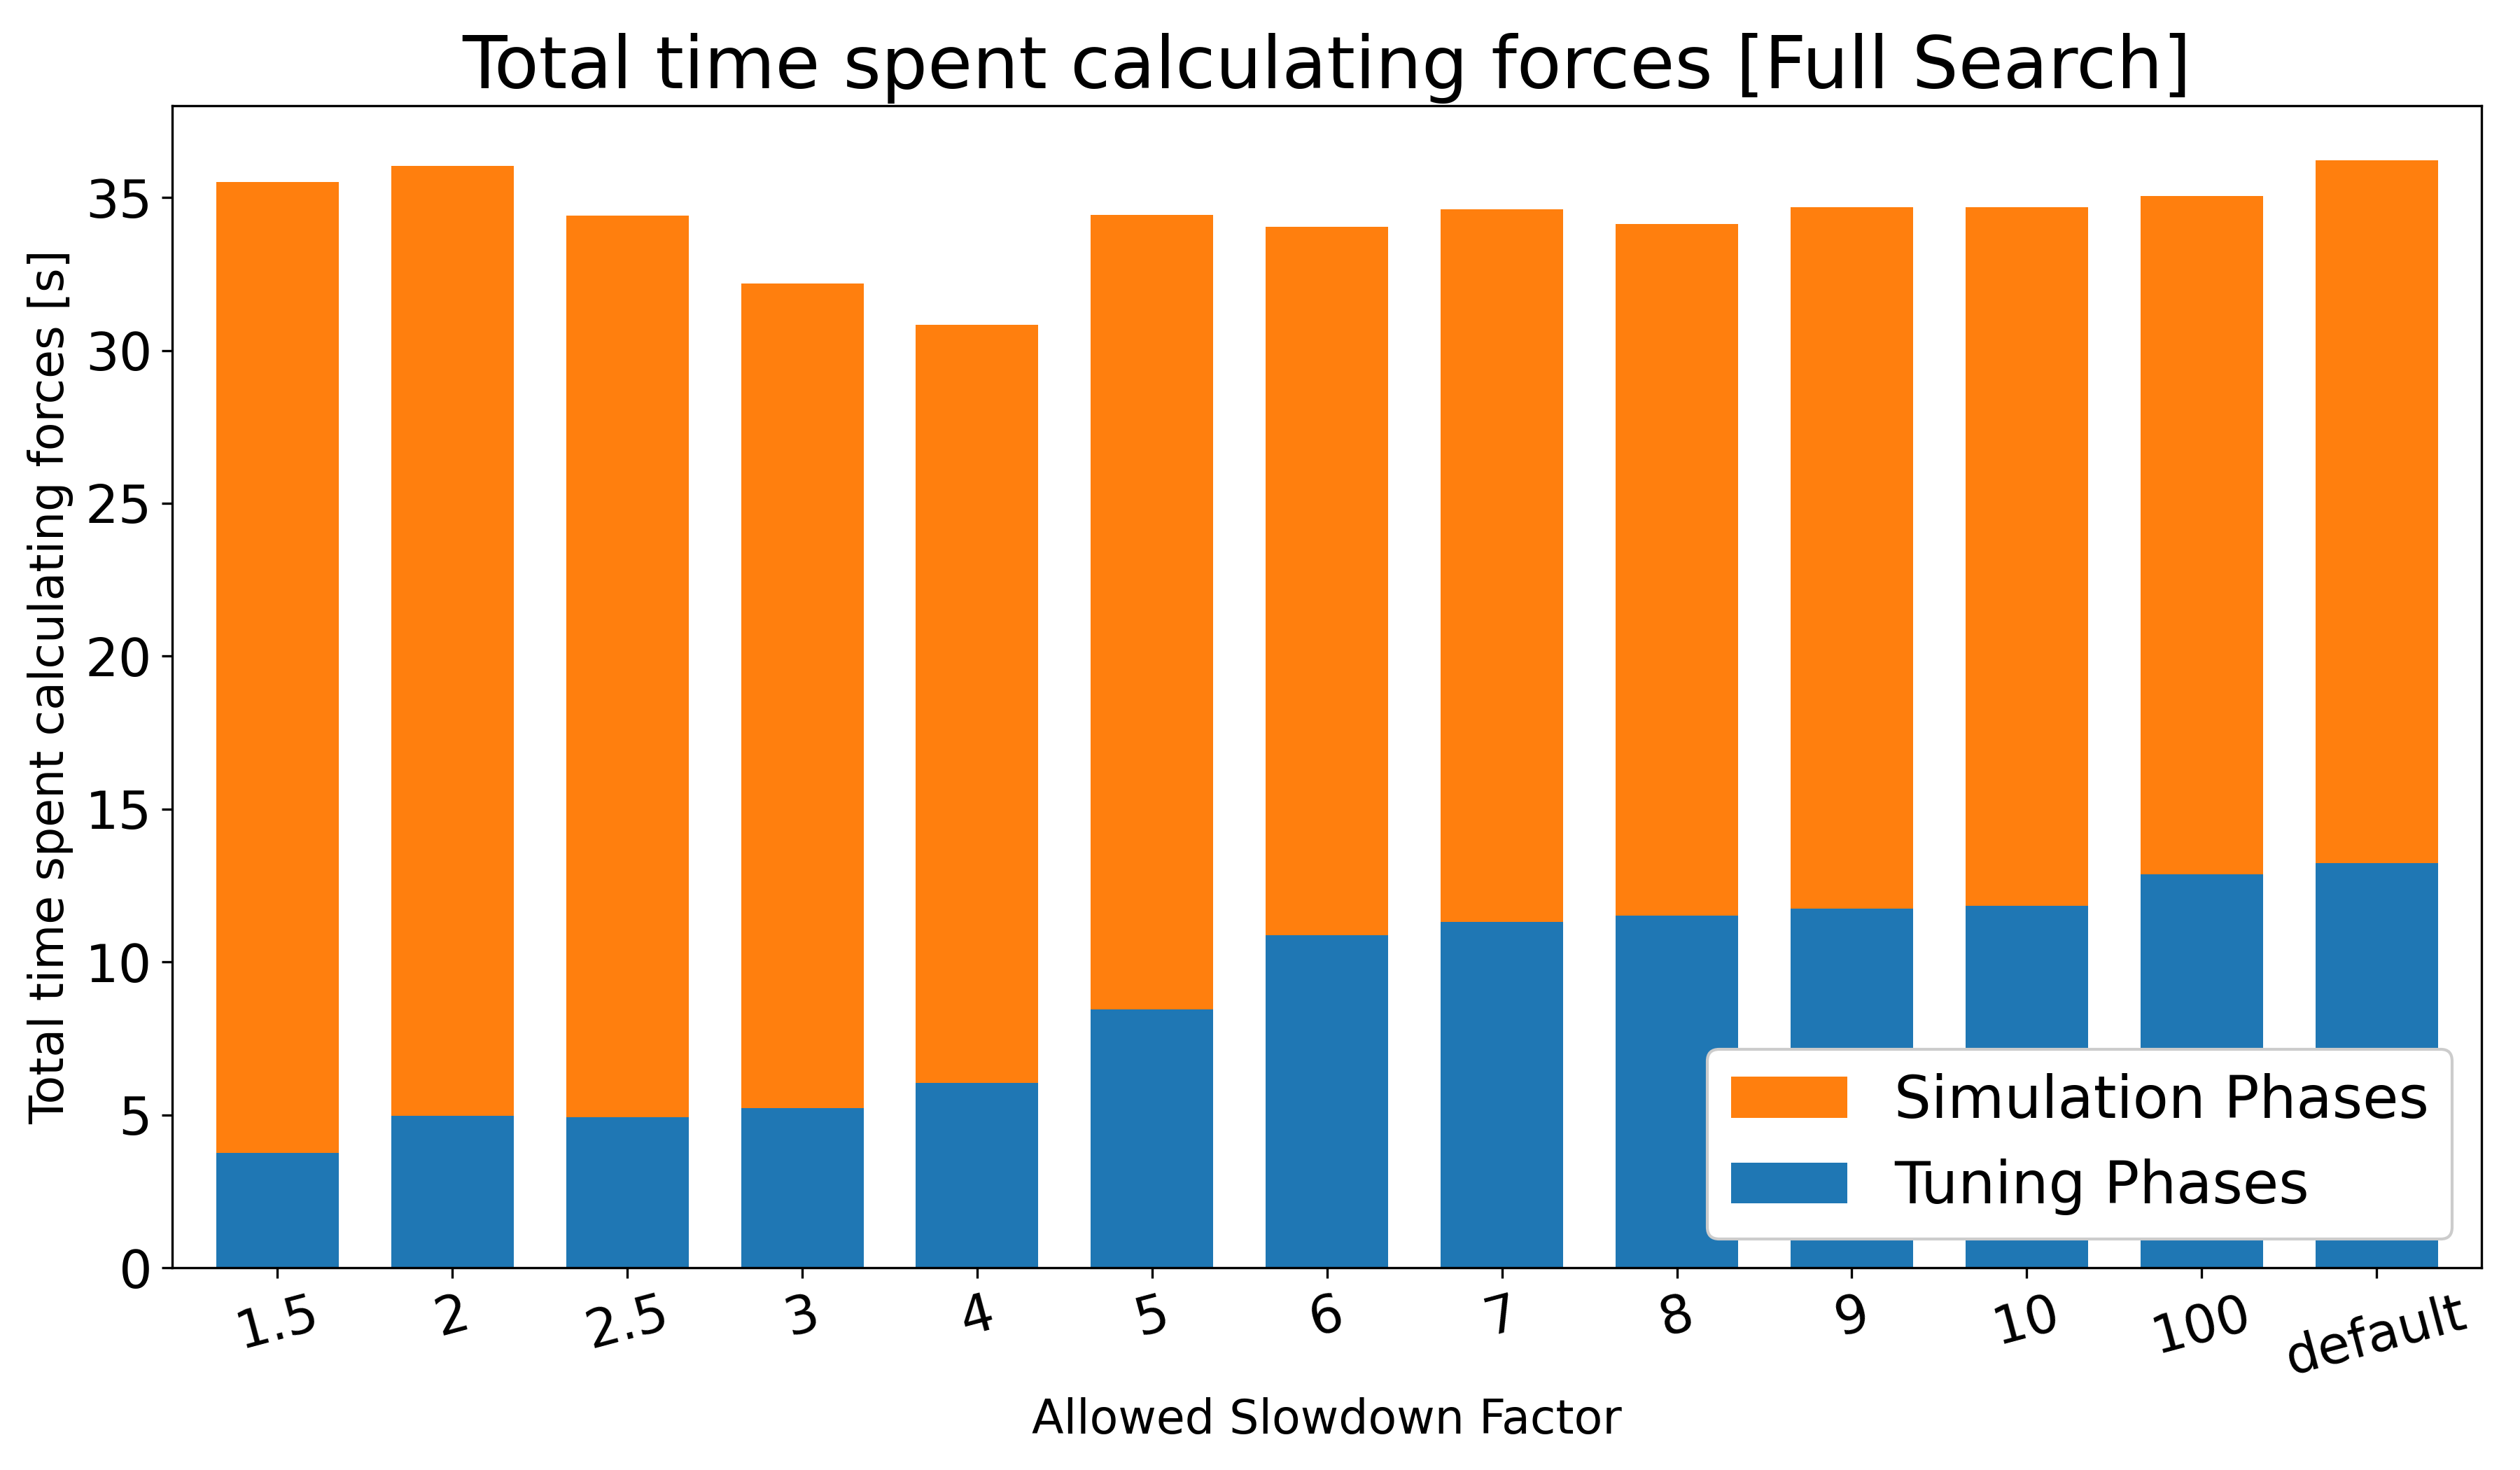
\includegraphics[width=\columnwidth]{../data/explodingLiquid/cluster/fullSearch/analytics/total_time_average.png}

    \caption{Total Simulation Time for Exploding Liquid Simulation with Early Stopping divided into tuning and simulation phases.}
    \label{fig:full_search}
\end{figure}


The total simulation time is minimal at a maximum allowed slowdown factor of $\approx4$ with a total simulation time of 30.84 seconds compared to 36.22 seconds without the early stopping mechanism. This is a reduction of 14.8\% in the total simulation time.

\subsubsection{Predictive Tuning}

The resulting performance when using the Predictive Tuning strategy in combination with the early stopping mechanism is shown in \autoref{fig:predictive_tuning}.

\begin{figure}[H]
    \centering

    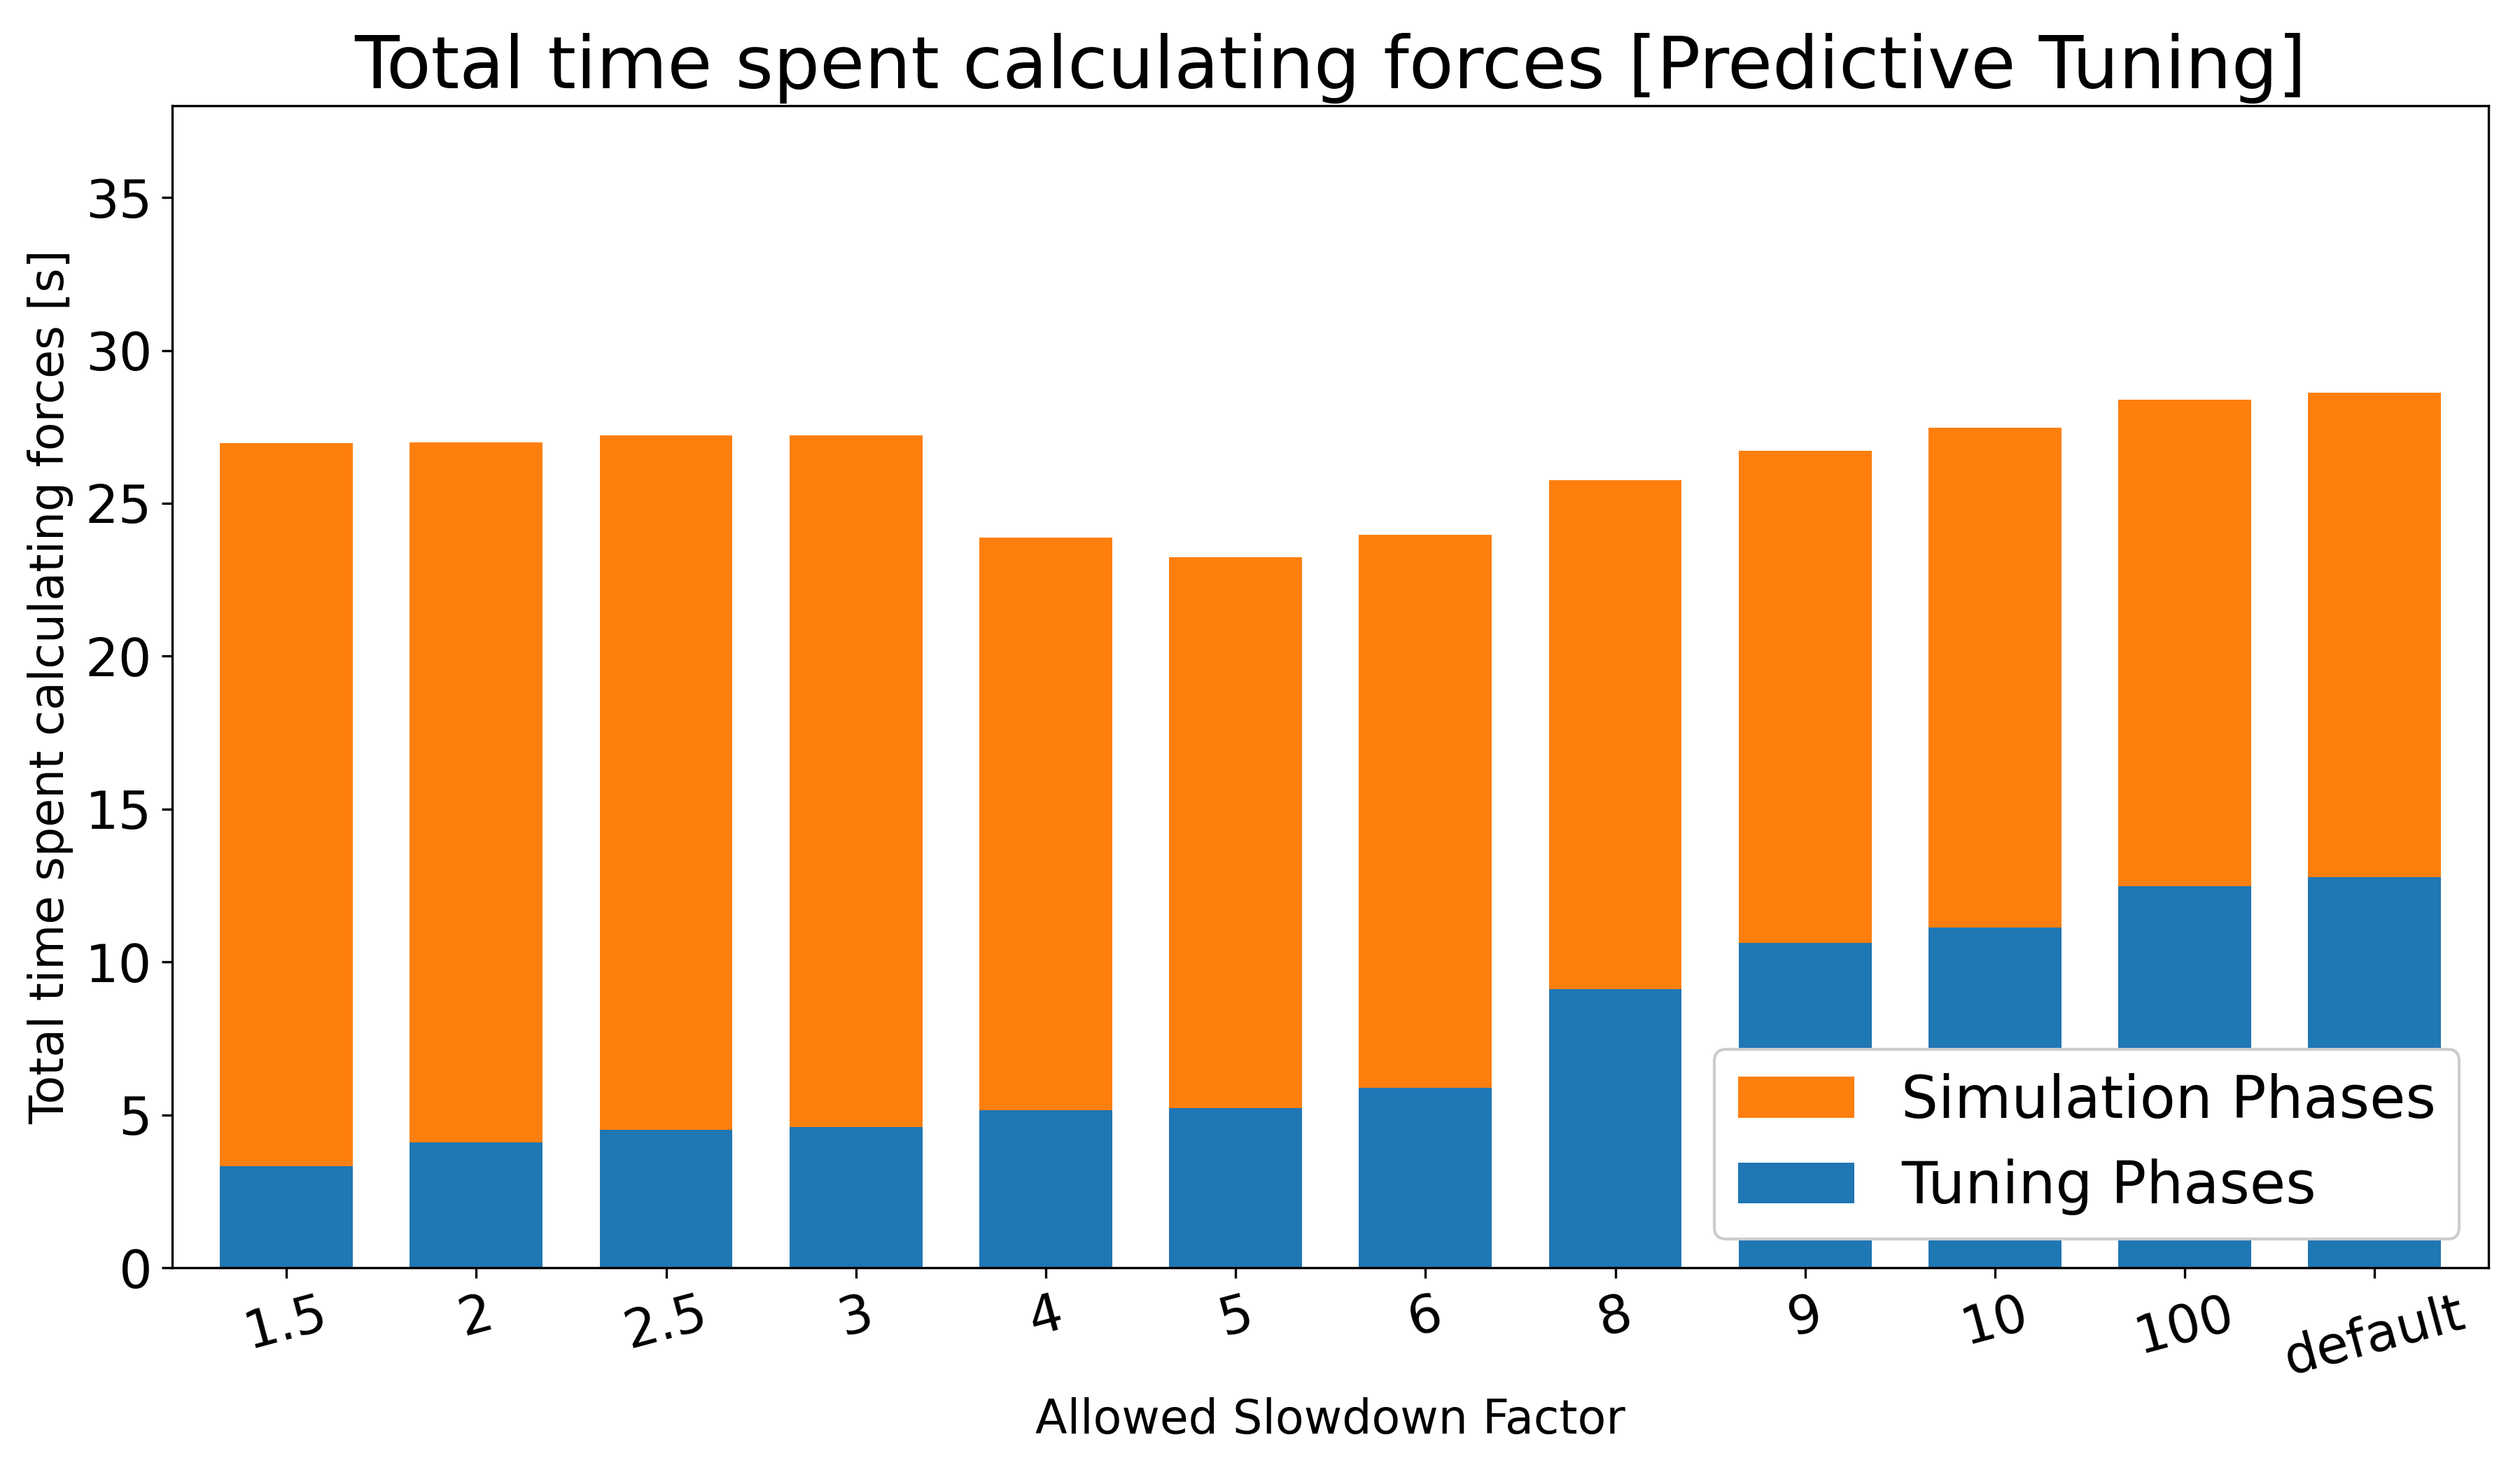
\includegraphics[width=\columnwidth]{../data/explodingLiquid/cluster/predictiveTuning/analytics/total_time_average.png}

    \caption{Total Simulation Time for Exploding Liquid Simulation with Early Stopping divided into tuning and simulation phases.}
    \label{fig:predictive_tuning}
\end{figure}


The total simulation time is minimal at a maximum allowed slowdown factor of $\approx5$ with a total simulation time of 23.23 seconds compared to 28.62 seconds without the early stopping mechanism. This is a reduction of 18.9\% in the total simulation time.

\subsection{Analysis and Discussion}

The evaluated benchmarks show that a slim range of thresholds capable of reducing the total simulation time exist for the \textit{Exploding Liquid} scenario.
Outside of this range, the total simulation time increases to levels comparable to the total simulation time without the early stopping mechanism. This is expected, as the two cases $maxAllowedSlowdown \to 1$ and $maxAllowedSlowdown \to \infty$ result in undesirable behavior: $maxAllowedSlowdown \to 1$ results in tuning phases with very few samples per configuration, as even small noise in the performance measurements causes the early stopping mechanism to abort the evaluation of a configuration, prohibiting reasonable estimates of the actual performance of a configuration. On the other hand, $maxAllowedSlowdown \to \infty$ results in the early stopping mechanism never aborting a configuration, which is equivalent to not using the early stopping mechanism at all. Picking a suitable threshold corresponds to finding a balance between the two extremes.

From the executed benchmarks, we deduce that the optimal threshold for the early stopping mechanism is around 4-5 for the \textit{Exploding Liquid} scenario. However, the optimal threshold probably varies between different simulation scenarios and tuning strategies, and further benchmarks are required to determine the optimal threshold for other scenarios.

The combination of the early stopping mechanism with good tuning strategies is beneficial, as good configurations are evaluated earlier resulting in a faster convergence of the fastest measured time, potentially resulting in more abortions of bad configurations.

It is noteworthy that the early stopping mechanism never caused a significant slowdown of the simulation, even when a low threshold was used.

We conclude that a naive implementation of the early stopping mechanism already provides a valuable addition to the AutoPas framework, as it can drastically reduce the total simulation time for certain scenarios, without causing significant overhead.


\section{Comparison with Other MD Engines}

Well-established MD engines such as GROMACS, LAMMPS, and ls1 mardyn have been developed over many years and achieve high performance in their respective use cases. This section provides a short overview of those engines and highlights the differences in their implementations.

\subsection{GROMACS}

Contrary to AutoPas, GROMACS only implements a single, highly optimized Verlet Cluster List scheme variant with flexible cluster sizes specifically designed for good SIMD vectorization.

Gromacs allows setting the vectorization parameters for the cluster size $M$ and the number of particles in neighbor groups $N$ statically to tune the force calculations to the SIMD width of the system~\cite{PALL20132641}. With suitable values for $M$ and $N$, computations of $M \times N$ particle interactions can be performed with just two SIMD load instructions~\cite{Solving_Software_Challenges_Exascale_2014}, drastically reducing the number of memory operations required for the force calculations and reaching up to 50\% of the peak flop rate on all supported hardware platforms~\cite{Solving_Software_Challenges_Exascale_2014}.

Gromacs defaults to $M=4$ and selects $N \in \{2, 4, 8\}$ depending on the SIMD width of the system. However, Finding good values is very time-consuming and depends on a detailed understanding of many low-level software optimization aspects of the different hardware platforms~\cite{PALL20132641}. In GROMACS, the developers have to manually tune this tuning.

\subsection{LAMMPS}

LAMMPS implements a single, highly optimized variant of the Verlet List scheme. The neighbor list is stored globally inside a multiple-page data structure. Inside each page, vectors of neighboring particles $J$ for multiple particles $I$ are stored inside a contiguous memory block~\cite{THOMPSON2022108171}, efficiently loading the neighbor list into the cache.
All particles are stored in a \textit{SoA} (Structure of Arrays) data layout~\cite{THOMPSON2022108171}.

LAMMPS supports accelerator packages using either CUDA, OpenCL, ROCm/HIP or OpenMP threads, hand-optimized
code, generically optimized code, and code using the KOKKOS library~\cite{Seckler2021}.


\subsection{ls1 mardyn}

ls1 mardyn differs from the previously mentioned MD engines as it uses the Linked Cells algorithm for particle interactions. Using LinkedCells provides a better memory efficiency than GROMACS and LAMMPS, allowing for simulations of massive particle systems~\cite{tchipev2019twe}. Internally, ls1 mardyn uses the default data layout of \textit{AoS} (Array of Structures) for the particle data. However, particular branches aimed at simulating massive particle systems can use a \texttt{RMM} (Reduced Memory Mode) layout in combination with a \textit{SoA} (Structure of Arrays) data layout, allowing for simulations of up to twenty trillion atoms~\cite{tchipev2019twe}.

To overcome the limitations of a single implementation, AutoPas was successfully integrated into ls1 mardyn, providing significant speedups in specific scenarios~\cite{SECKLER2021101296}.


\section{Conclusion}

\todo{conclusion}


\bibliographystyle{IEEEtran}
\bibliography{literature}



\newpage
\newpage
\tableofcontents

\end{document}

